\question The figure shows a section of wire connected to a battery. Every part of the wire is made of the same material and has the same cross-sectional area. The circuit is in the steady state.

\begin{figure}[ht!]
	\centering
	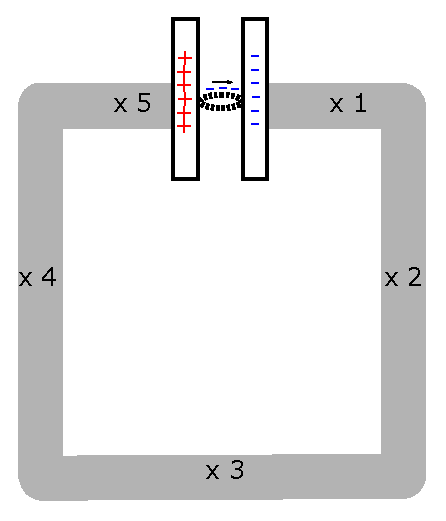
\includegraphics[width=8cm]{battery}
\end{figure}

\begin{parts}
	\part On the figure (or on your own copy of the figure): sketch (using arrows) the electric field $\vec{E}$, electron current $i$, and drift velocity $v$ at each labeled location of the circuit. Be sure that your arrows indicate direction and relative magnitude.
	\part In locations 2-5 of the wire, how does the electron current $i$ compare to the current at location 1 ($i_1$)? (Equal to, less than, greater than)
	\vspace{1cm}
	\part In locations 2-5 of the wire, how does the drift velocity $v$ compare to the drift velocity at location 1 ($v_1)$? 
	\vspace{1cm}
	\part In locations 2-5 of the wire, how does the magnitude of the electric field $E$ compare to the magnitude of the field at location 1 ($E_1$)?
	\vspace{1cm}
	\part We can approximately treat the battery as an electric dipole, which has a weaker electric field at greater distances ($|\vec{E}_\mathrm{batt}|\propto 1/r^3$). Is your result from part (d) consistent with the electric field of a dipole? If not, explain the discrepancy.
	\vspace{1cm}
	\part Suppose the wire in this circuit is a 10-cm long copper wire with a cross-sectional area of $2\times 10^{-5}$ m$^2$. For copper: the mobile electron density is $8.5\times10^{28}$ electrons per m$^3$, and the electron mobility is 4.5$\times10^{-3}\frac{\mathrm{m/s}}{\mathrm{N/C}}$. If the battery has an emf $\varepsilon=3$ V, what is the drift velocity of the moving electrons at location 3?
\end{parts}